%%=====================================================================
%% Apresentação do TCC — padrão UDESC (tema beamerthemeUDESC.sty)
%%
%%   make            (ou: pdflatex apresentacao.tex, duas passadas)
%%
%% As figuras são lidas direto de ../Textual/Textuais/Imgs, sem cópia.
%% Slides com a etiqueta "RESULTADO ILUSTRATIVO" trazem conteúdo
%% provisório: substituir pelos dados reais antes da defesa.
%%=====================================================================
\documentclass[aspectratio=169,11pt]{beamer}

\usepackage[utf8]{inputenc}
\usepackage[T1]{fontenc}
\usepackage{lmodern}
\usepackage[brazil]{babel}
\usepackage{amsmath}
\usepackage{booktabs}
\usepackage{siunitx}
\sisetup{output-decimal-marker={,}}

\usetheme[semtrilha]{UDESC}

\graphicspath{{../Textual/Textuais/Imgs/}}

% marca de conteúdo provisório (resultado ilustrativo)
\newcommand{\ilustrativo}{%
  \begin{tikzpicture}[remember picture, overlay]
    \node[anchor=north east, fill=udescvermelhoB, text=white,
          font=\tiny\bfseries, inner sep=3pt, rounded corners=2pt]
      at ([xshift=-0.6cm, yshift=-0.45cm]current page.north east)
      {RESULTADO ILUSTRATIVO};
  \end{tikzpicture}}

%%---------------------------------------------------------------------
\title{Bancada de Medição para Sistemas Propulsivos Elétricos com Motor BLDC}
\subtitulo{Trabalho de Conclusão de Curso\\Engenharia Elétrica}
\author{Vitor Dall'Olivo Gonçalves}
\orientador{Prof.\textsuperscript{a} Ana Teruko Yokomizo Watanabe}
\coorientador{Aureo Guilherme Dobrikopf}
\local{Joinville, 2026}

\begin{document}

\capaudesc

%%=====================================================================
%% INTRODUÇÃO: contexto, problema, conjugado da hélice, objetivos
%%=====================================================================
\begin{frame}{Albatroz Aerodesign}
  \begin{columns}[c]
    \begin{column}{0.42\textwidth}
      \begin{itemize}
        \item Competição SAE Brasil Aerodesign
        \item Motor BLDC obrigatório
        \item Propulsão define a carga útil
      \end{itemize}
    \end{column}
    \begin{column}{0.58\textwidth}
      \centering
      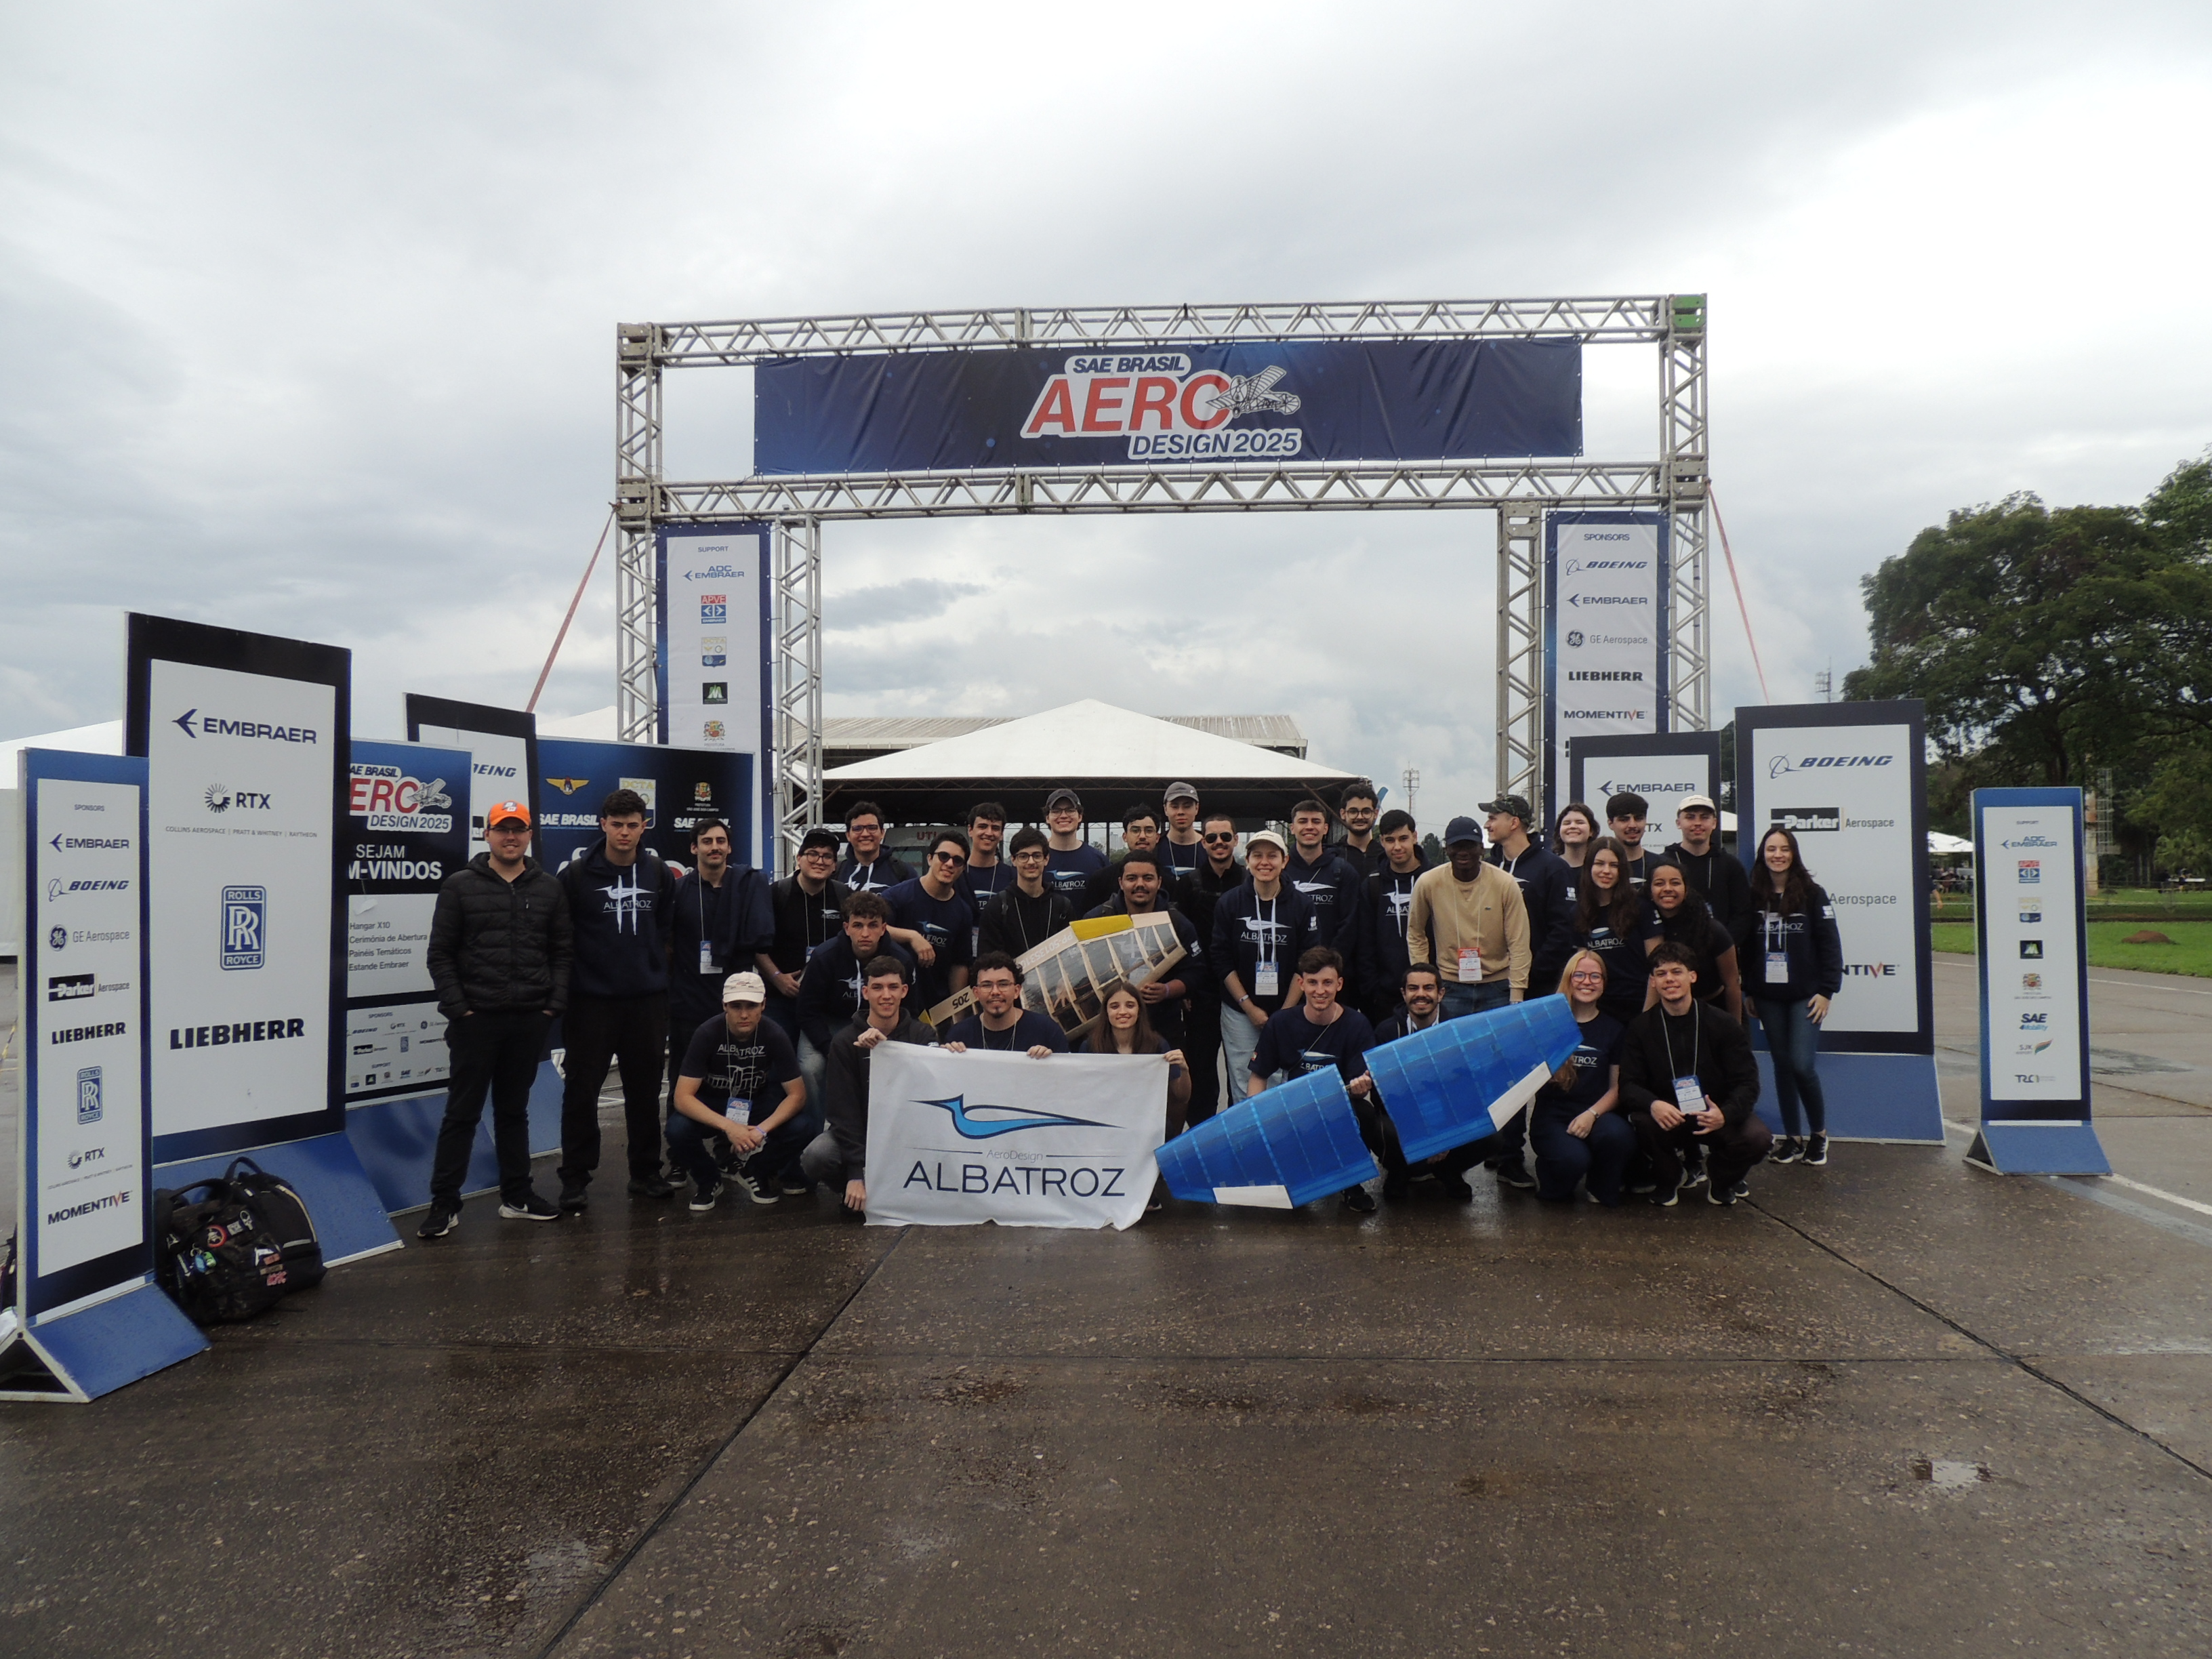
\includegraphics[width=\linewidth]{Introducao/DSCN3474.JPG}
      \fonte[Equipe Albatroz; SAE Brasil (2024)]
    \end{column}
  \end{columns}
\end{frame}

\begin{frame}{Ensaios descentralizados}
  \begin{columns}[c]
    \begin{column}{0.4\textwidth}
      \centering
      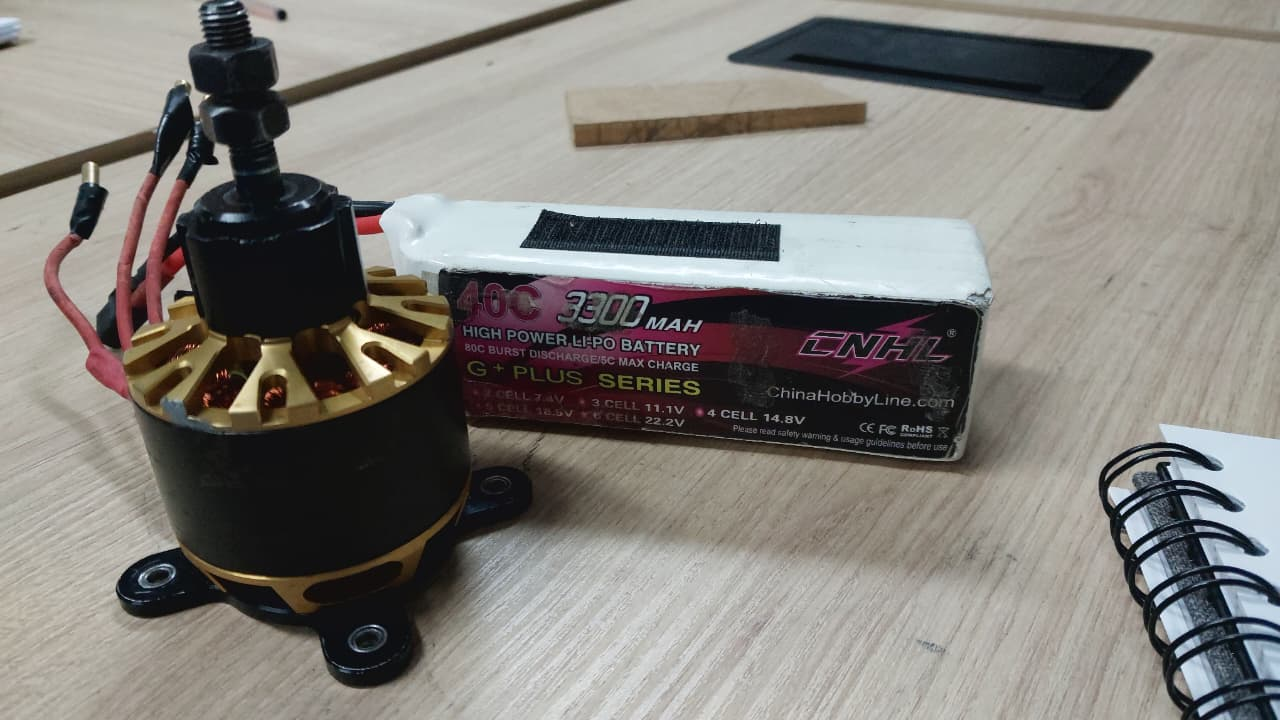
\includegraphics[height=0.5\textheight]{Metodologia/Motor_batata.jpeg}\\[0.3em]
      {\small Motor e bateria}
    \end{column}
    \begin{column}{0.6\textwidth}
      \centering
      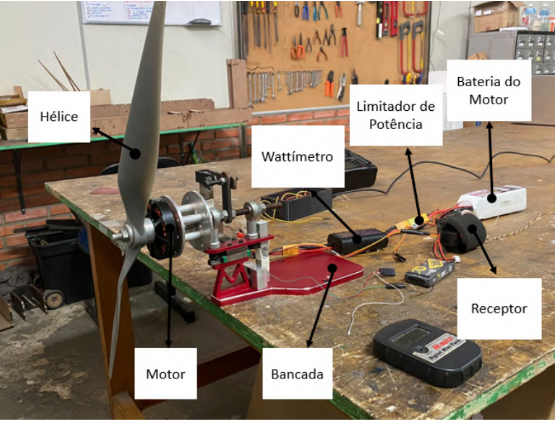
\includegraphics[height=0.5\textheight]{Introducao/BancadaDesempenho.png}\\[0.3em]
      {\small Bancada atual}
    \end{column}
  \end{columns}
  \destaque{Sem medida direta de rotação e torque: só estimativas.}
  \fonte[Autor; Souza e Veber (2023); Costa (2021)]
\end{frame}

\begin{frame}{Conjugado da hélice}
  \[ Q = C_Q\,\rho\,n^2 D^5 \]
  \begin{columns}[c]
    \begin{column}{0.5\textwidth}
      \centering
      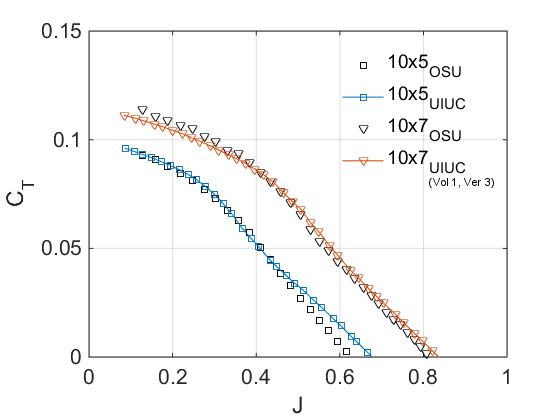
\includegraphics[height=0.5\textheight]{Revisao/Selig_propeller_data_ct.png}
    \end{column}
    \begin{column}{0.5\textwidth}
      \centering
      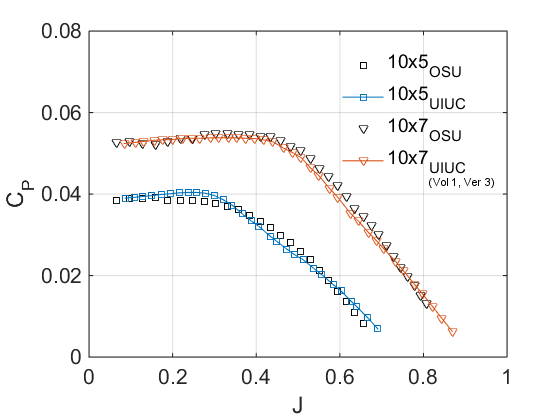
\includegraphics[height=0.5\textheight]{Revisao/Selig_propeller_data_cp.png}
    \end{column}
  \end{columns}
  \fonte[McCrink e Gregory (2015); McCormick (1995)]
\end{frame}

\begin{frame}{Torque define o envelope}
  \begin{columns}[c]
    \begin{column}{0.36\textwidth}
      Hélices de referência
      \begin{itemize}
        \item APC 15x6E
        \item APC 17x10E
      \end{itemize}
      \vspace{0.5em}
      Simuladas com o catálogo e ensaiadas em bancada
    \end{column}
    \begin{column}{0.64\textwidth}
      \centering
      \tikzfig{1}{0.7}{helice_ponto_op}
      \fonte[Autor; APC Propellers (2026); Brandt et al.\ (2015)]
    \end{column}
  \end{columns}
\end{frame}

\begin{frame}{Objetivos}
  \destaque{Desenvolver um sistema integrado de aquisição de dados,
            adaptando a bancada de ensaios motopropulsores da equipe.}

  \vspace{0.6em}
  \begin{itemize}
    \item Sistema de medição do motor BLDC
    \item Modelo do motor e observador de estados
    \item Medição aerodinâmica da hélice
    \item Rede Ethernet entre os nós e o supervisório
    \item Software de supervisão em Python
  \end{itemize}
\end{frame}

%%=====================================================================
%% METODOLOGIA
%%=====================================================================
\secaoudesc{Metodologia}

\begin{frame}{Arquitetura}
  \begin{columns}[c]
    \begin{column}{0.38\textwidth}
      \begin{itemize}
        \item \alert{SIBA}: aerodinâmica e bateria
        \item \alert{SAME}: tensões e correntes do motor
        \item Supervisório via TCP/UDP
      \end{itemize}
    \end{column}
    \begin{column}{0.62\textwidth}
      \centering
      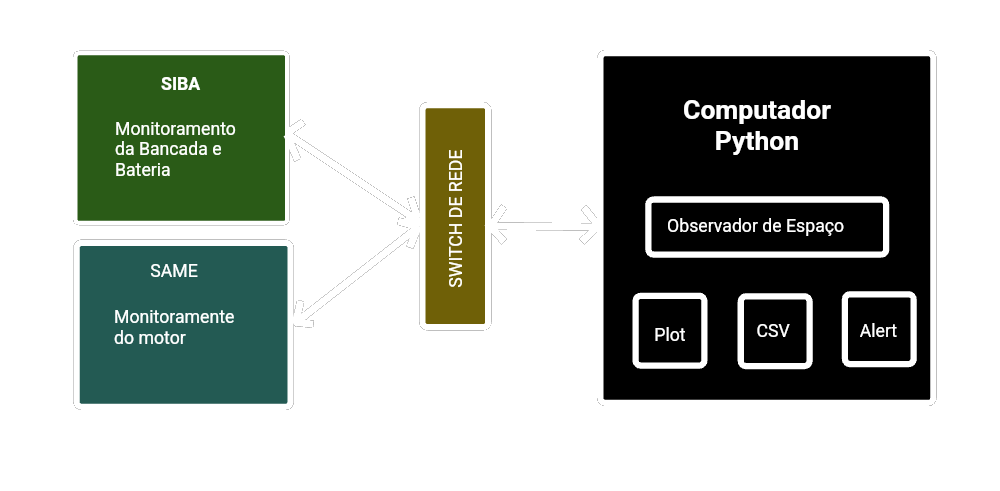
\includegraphics[width=\linewidth]{Metodologia/Arquitetura.png}
      \fonte[Autor; An (2026)]
    \end{column}
  \end{columns}
\end{frame}

\begin{frame}{Modelo do motor}
  \[
    \begin{bmatrix} v_\alpha \\ v_\beta \end{bmatrix}
    = R_s \begin{bmatrix} i_\alpha \\ i_\beta \end{bmatrix}
    + L_s \frac{\mathrm{d}}{\mathrm{d}t}
      \begin{bmatrix} i_\alpha \\ i_\beta \end{bmatrix}
    + \begin{bmatrix} e_\alpha \\ e_\beta \end{bmatrix}
  \]
  \[
    \hat{T}_e = \frac{3p}{4\,\hat{\omega}_e}
      \left(\hat{e}_\alpha i_\alpha + \hat{e}_\beta i_\beta\right)
  \]
  \fonte[Clarke (1943); Fitzgerald, Kingsley e Umans (2014); Krishnan (2017)]
\end{frame}

\begin{frame}{Observador por modos deslizantes}
  \begin{columns}[c]
    \begin{column}{0.36\textwidth}
      \begin{itemize}
        \item SMO estima a FEM
        \item PLL extrai ângulo e velocidade
        \item Reconstrução analítica da FEM
      \end{itemize}
    \end{column}
    \begin{column}{0.64\textwidth}
      \centering
      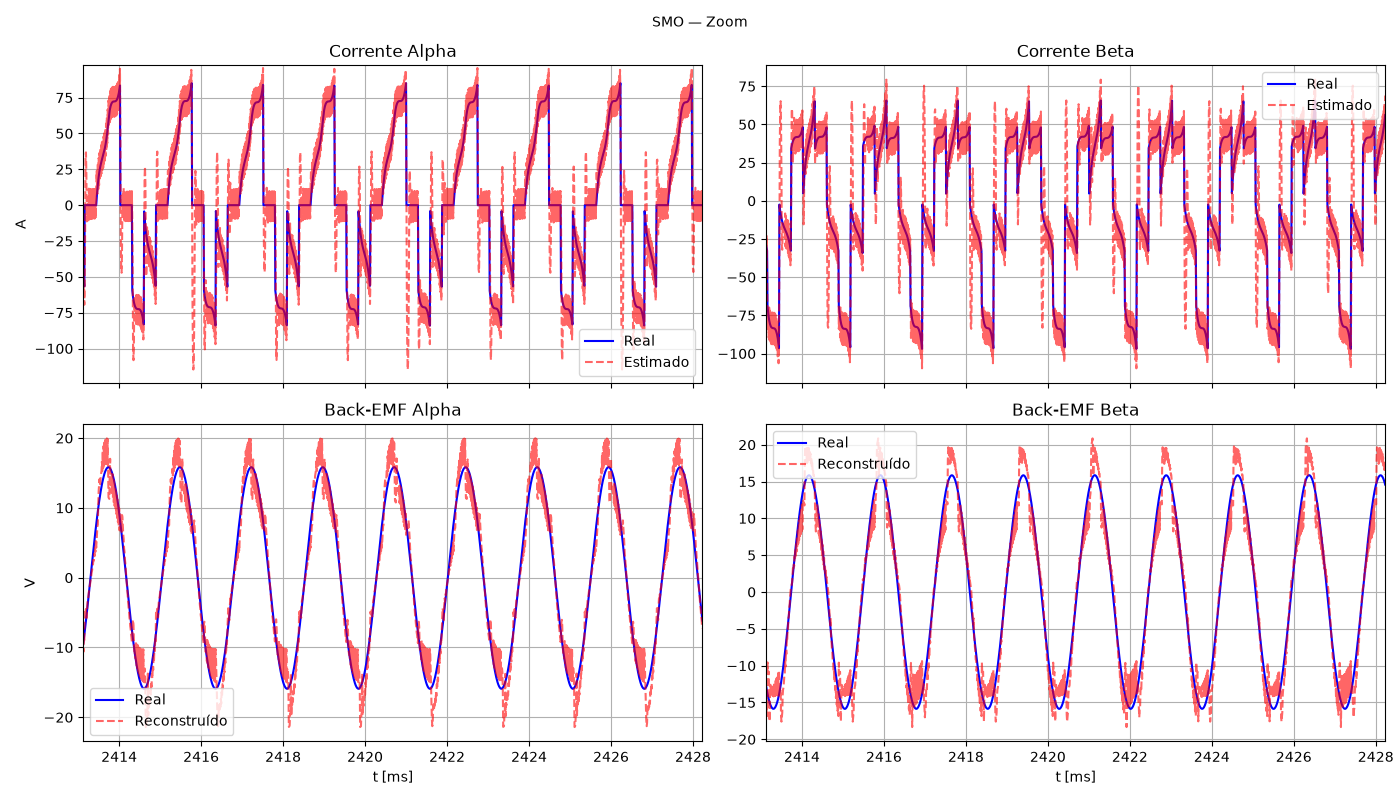
\includegraphics[width=\linewidth]{Desenvolvimento/reconstrucao_backemf.png}
      \fonte[Adaptado de Utkin (1992); Young, Utkin e Özgüner (1999); Abo Kaf et al.\ (2024)]
    \end{column}
  \end{columns}
\end{frame}

\begin{frame}{Ajuste automático dos ganhos}
  \begin{columns}[c]
    \begin{column}{0.36\textwidth}
      \begin{itemize}
        \item Evolução Diferencial
        \item Custo: torque + rotação
        \item Ganhos independentes do passo de amostragem
      \end{itemize}
    \end{column}
    \begin{column}{0.64\textwidth}
      \centering
      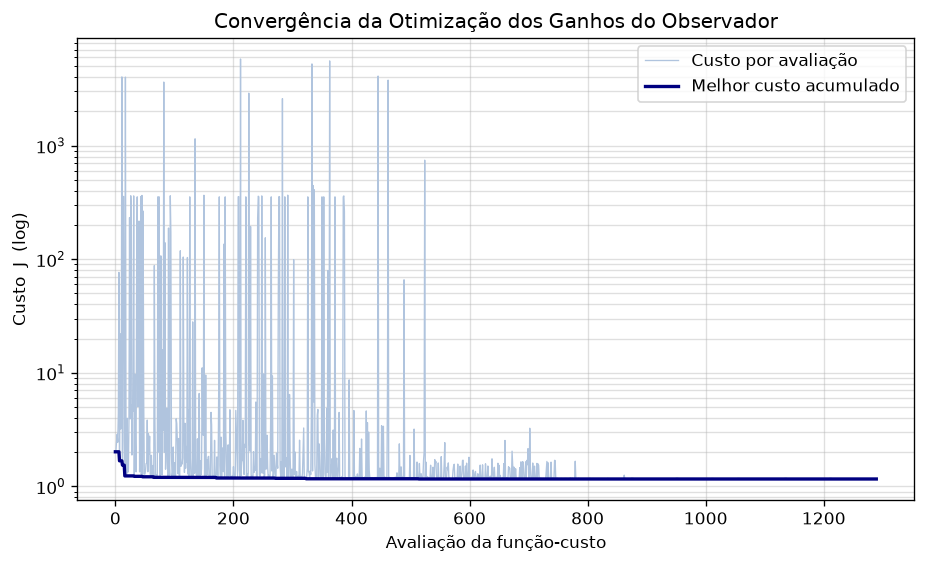
\includegraphics[width=\linewidth]{Desenvolvimento/Otim_convergencia.png}
      \fonte[Autor; Slotine e Li (1991)]
    \end{column}
  \end{columns}
\end{frame}

\begin{frame}{Hardware}
  \centering
  \begin{columns}[t]
    \begin{column}{0.33\textwidth}
      \centering
      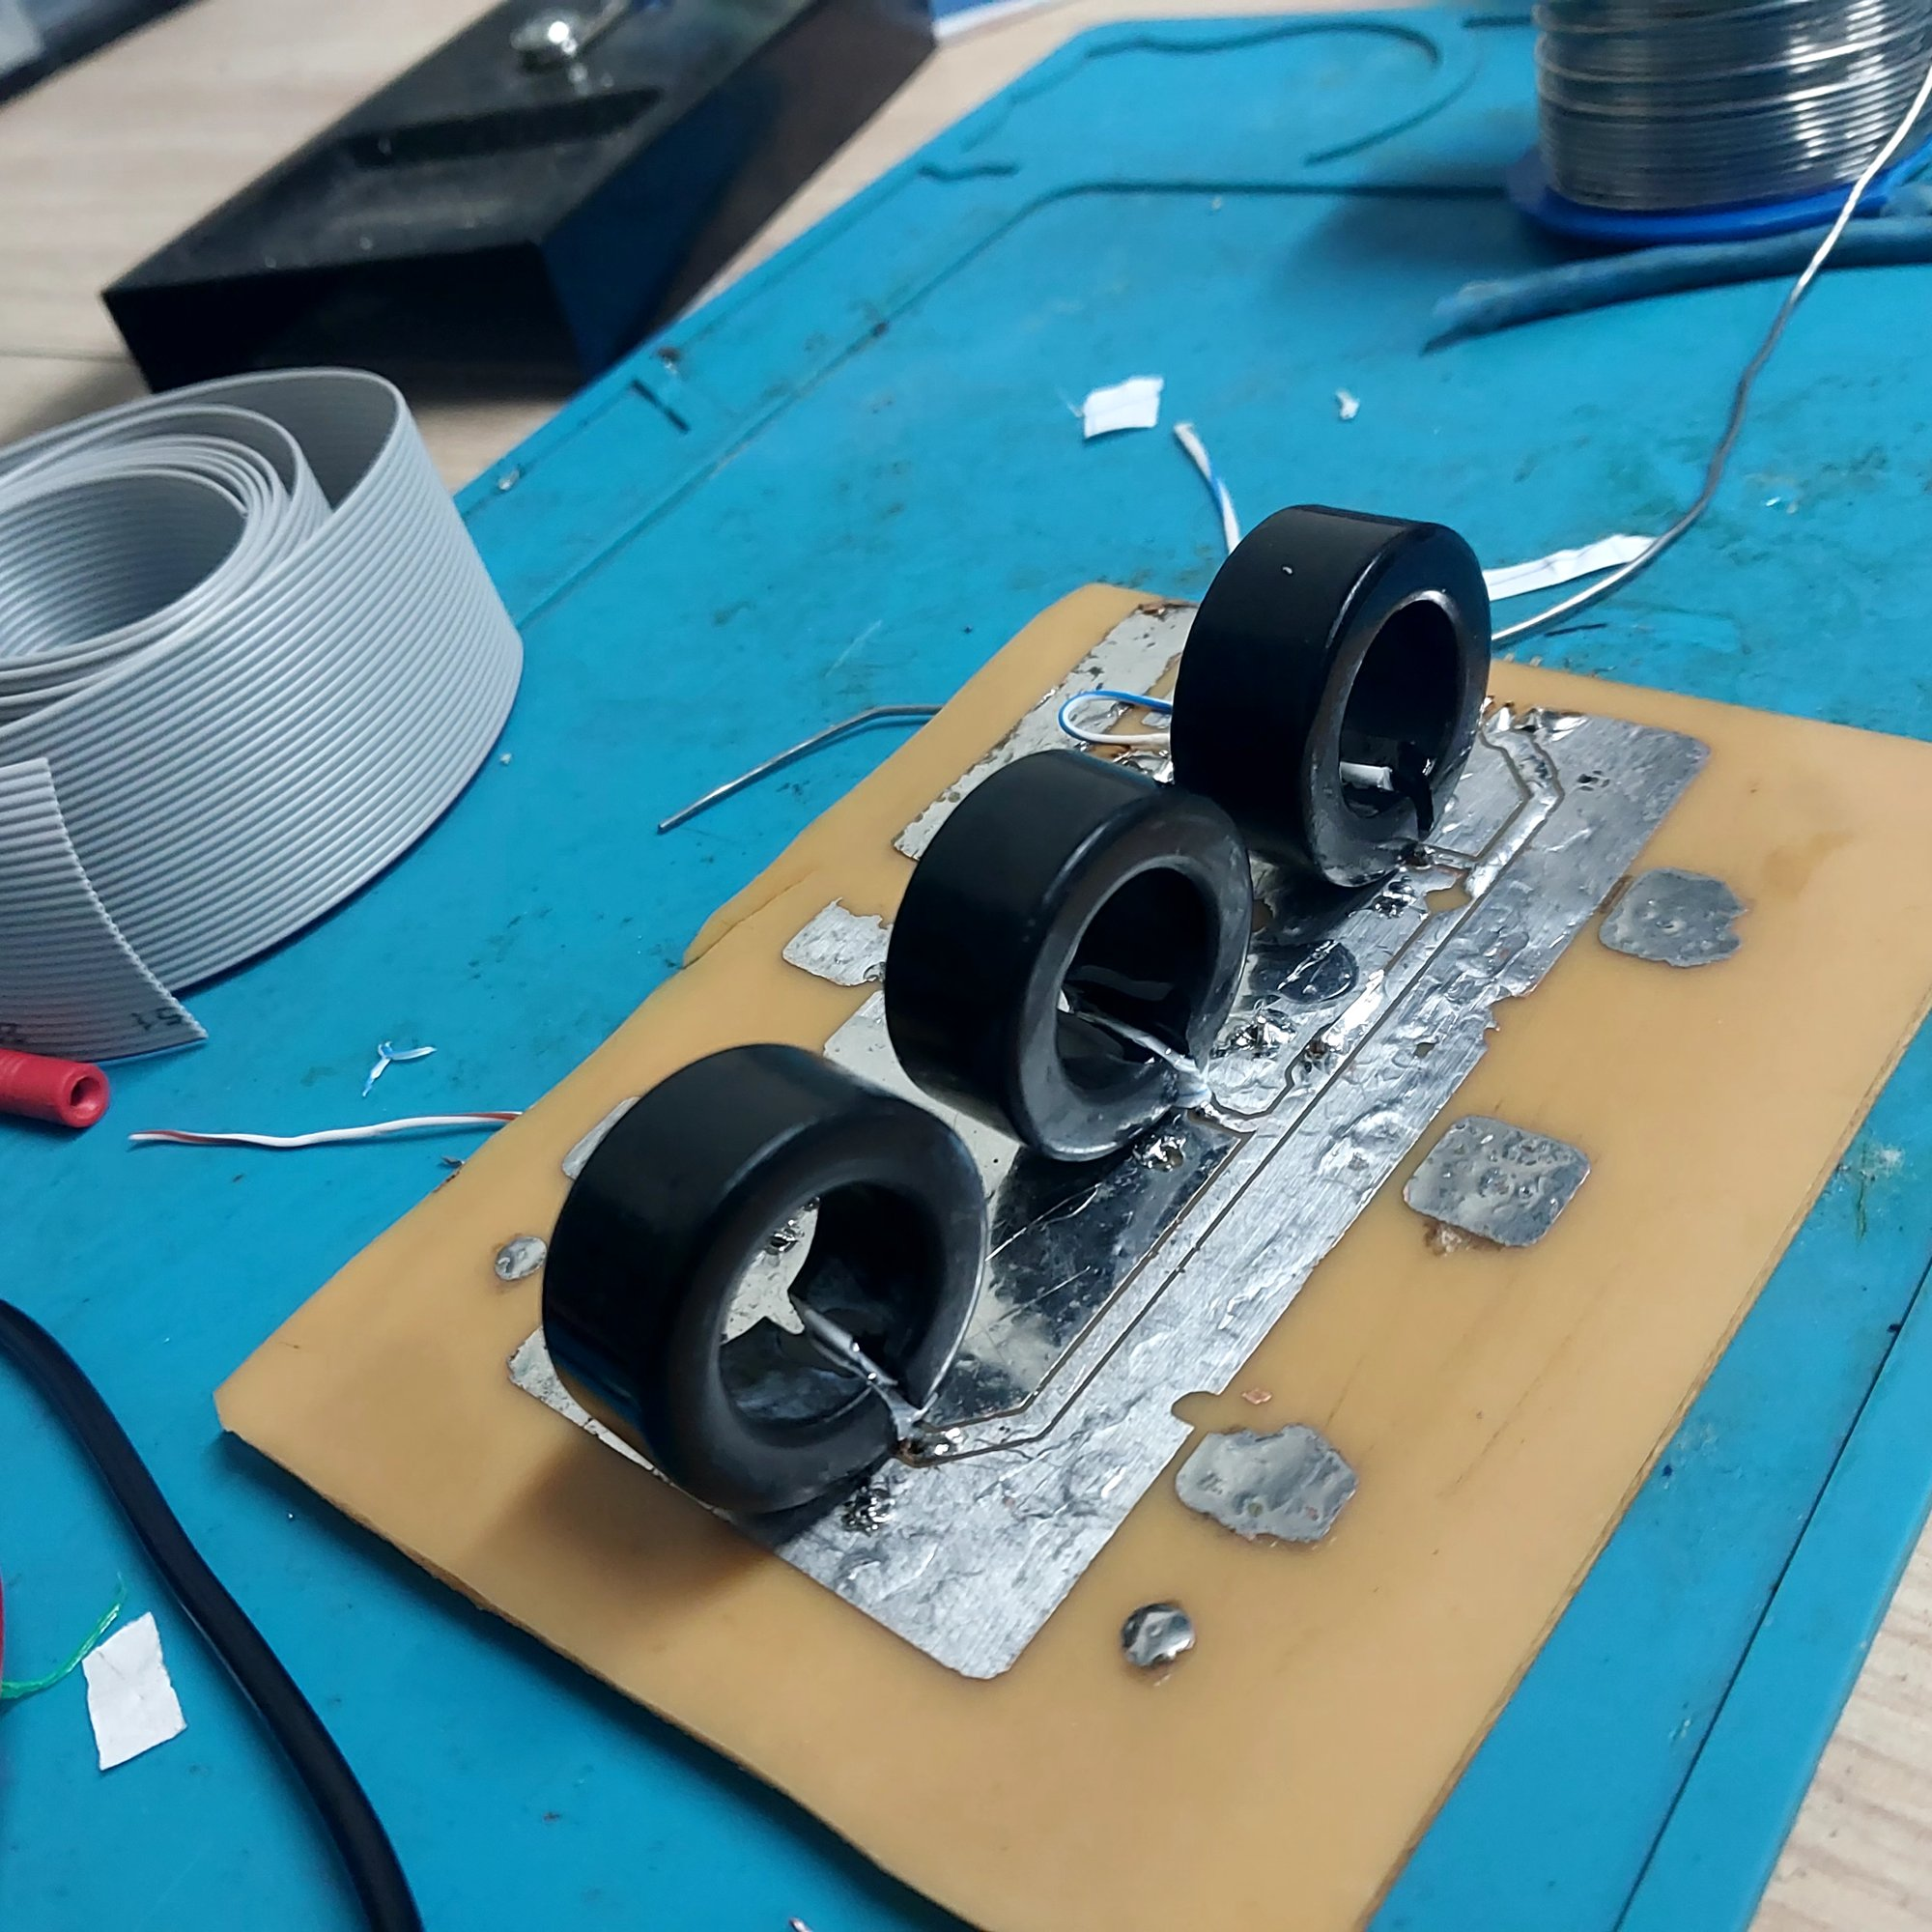
\includegraphics[height=0.5\textheight,width=0.95\linewidth,keepaspectratio]{Resultados/pcb_feita_aq1.jpg}\\[0.3em]
      {\small Placa AQ1}
    \end{column}
    \begin{column}{0.33\textwidth}
      \centering
      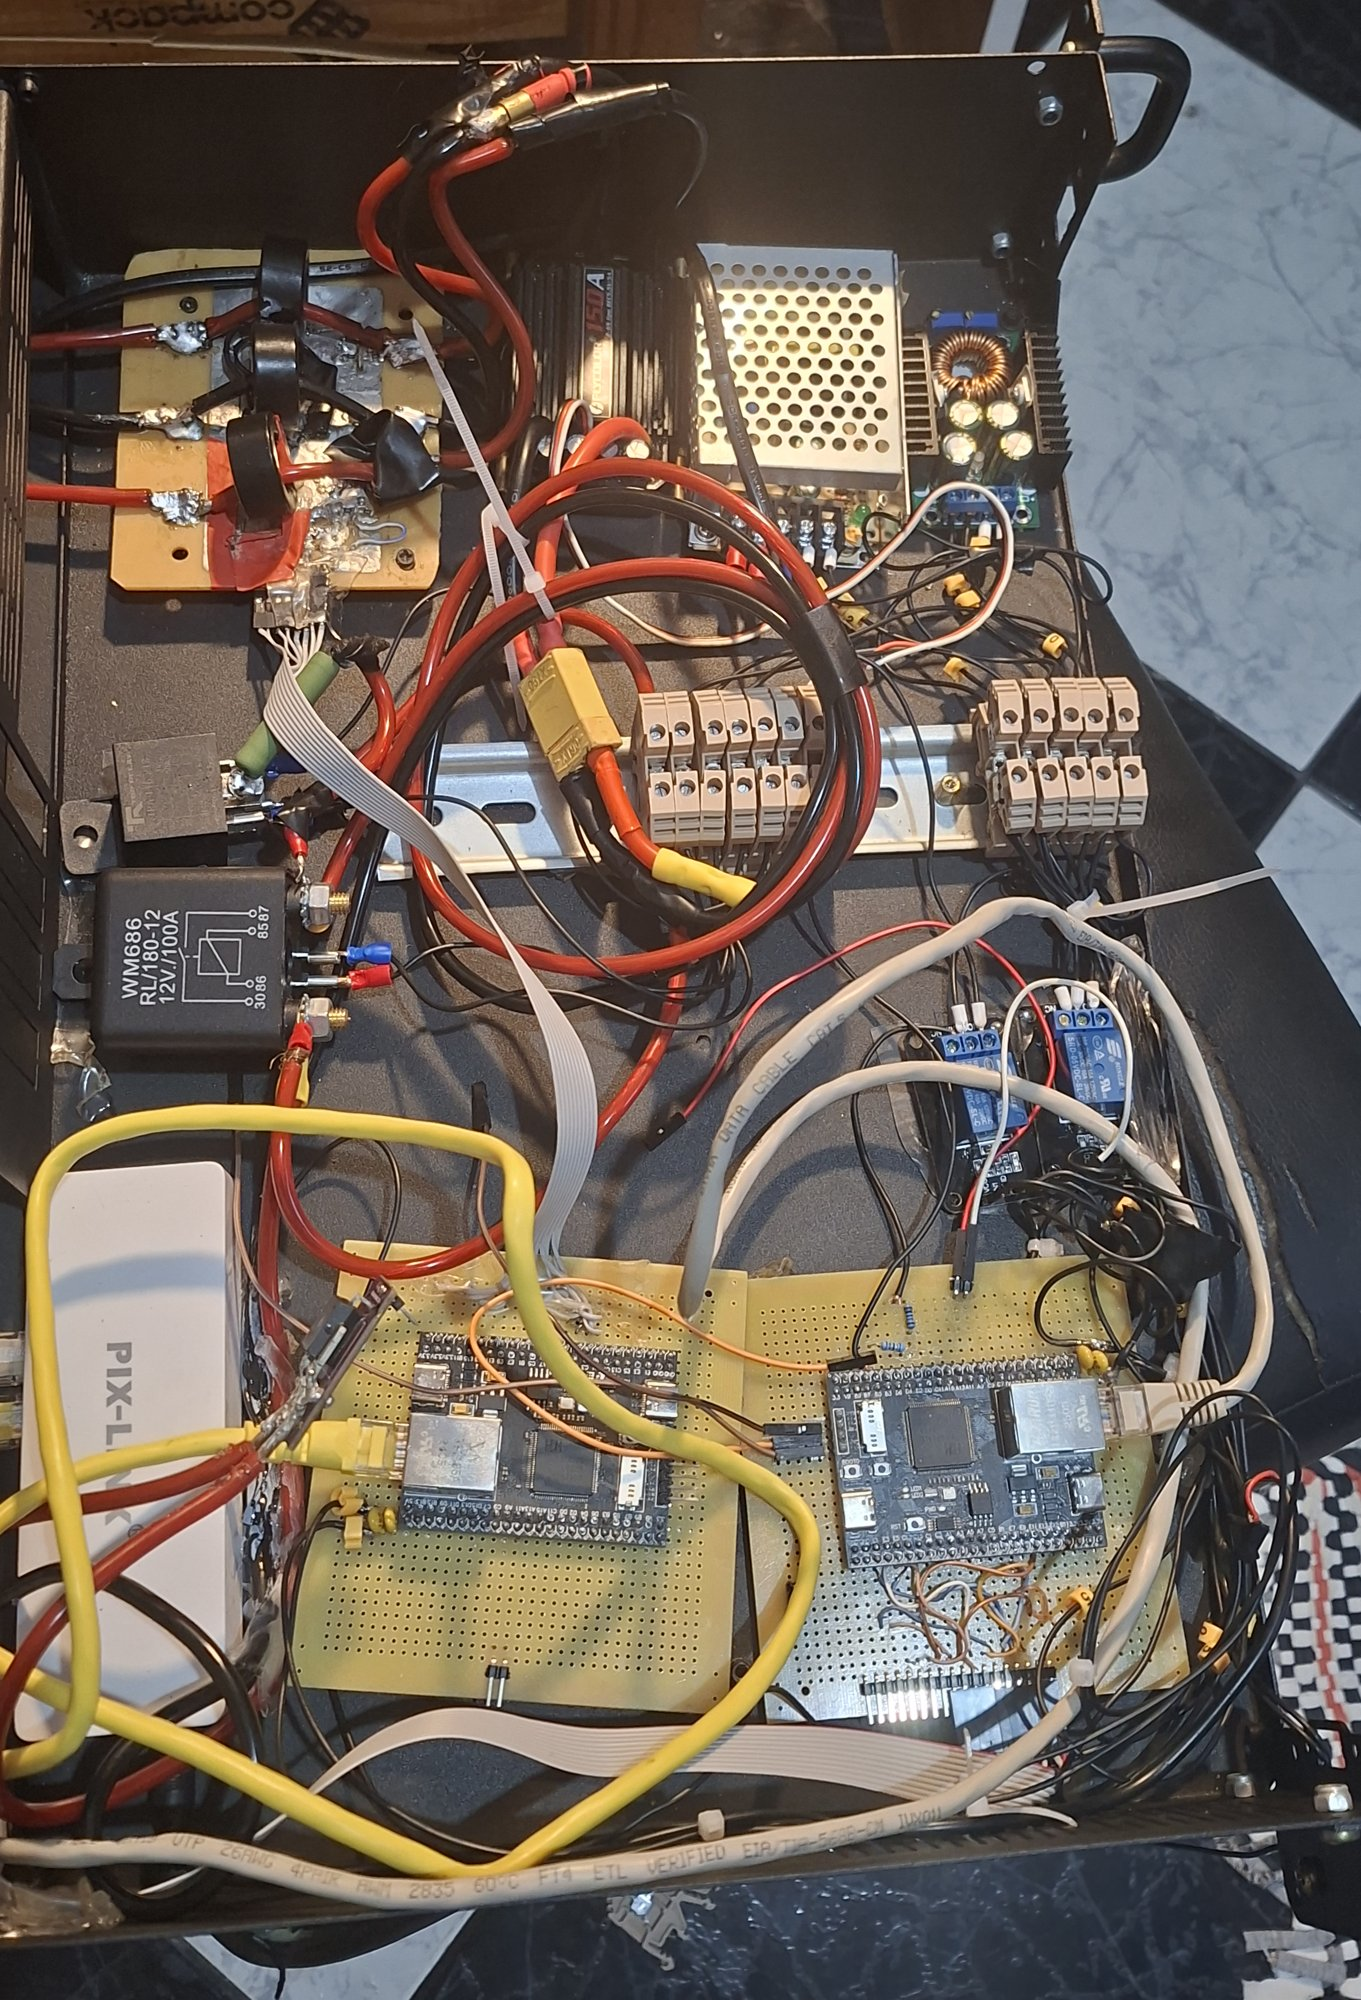
\includegraphics[height=0.5\textheight,width=0.95\linewidth,keepaspectratio]{Resultados/montagem_finalizada.jpg}\\[0.3em]
      {\small Fiação}
    \end{column}
    \begin{column}{0.33\textwidth}
      \centering
      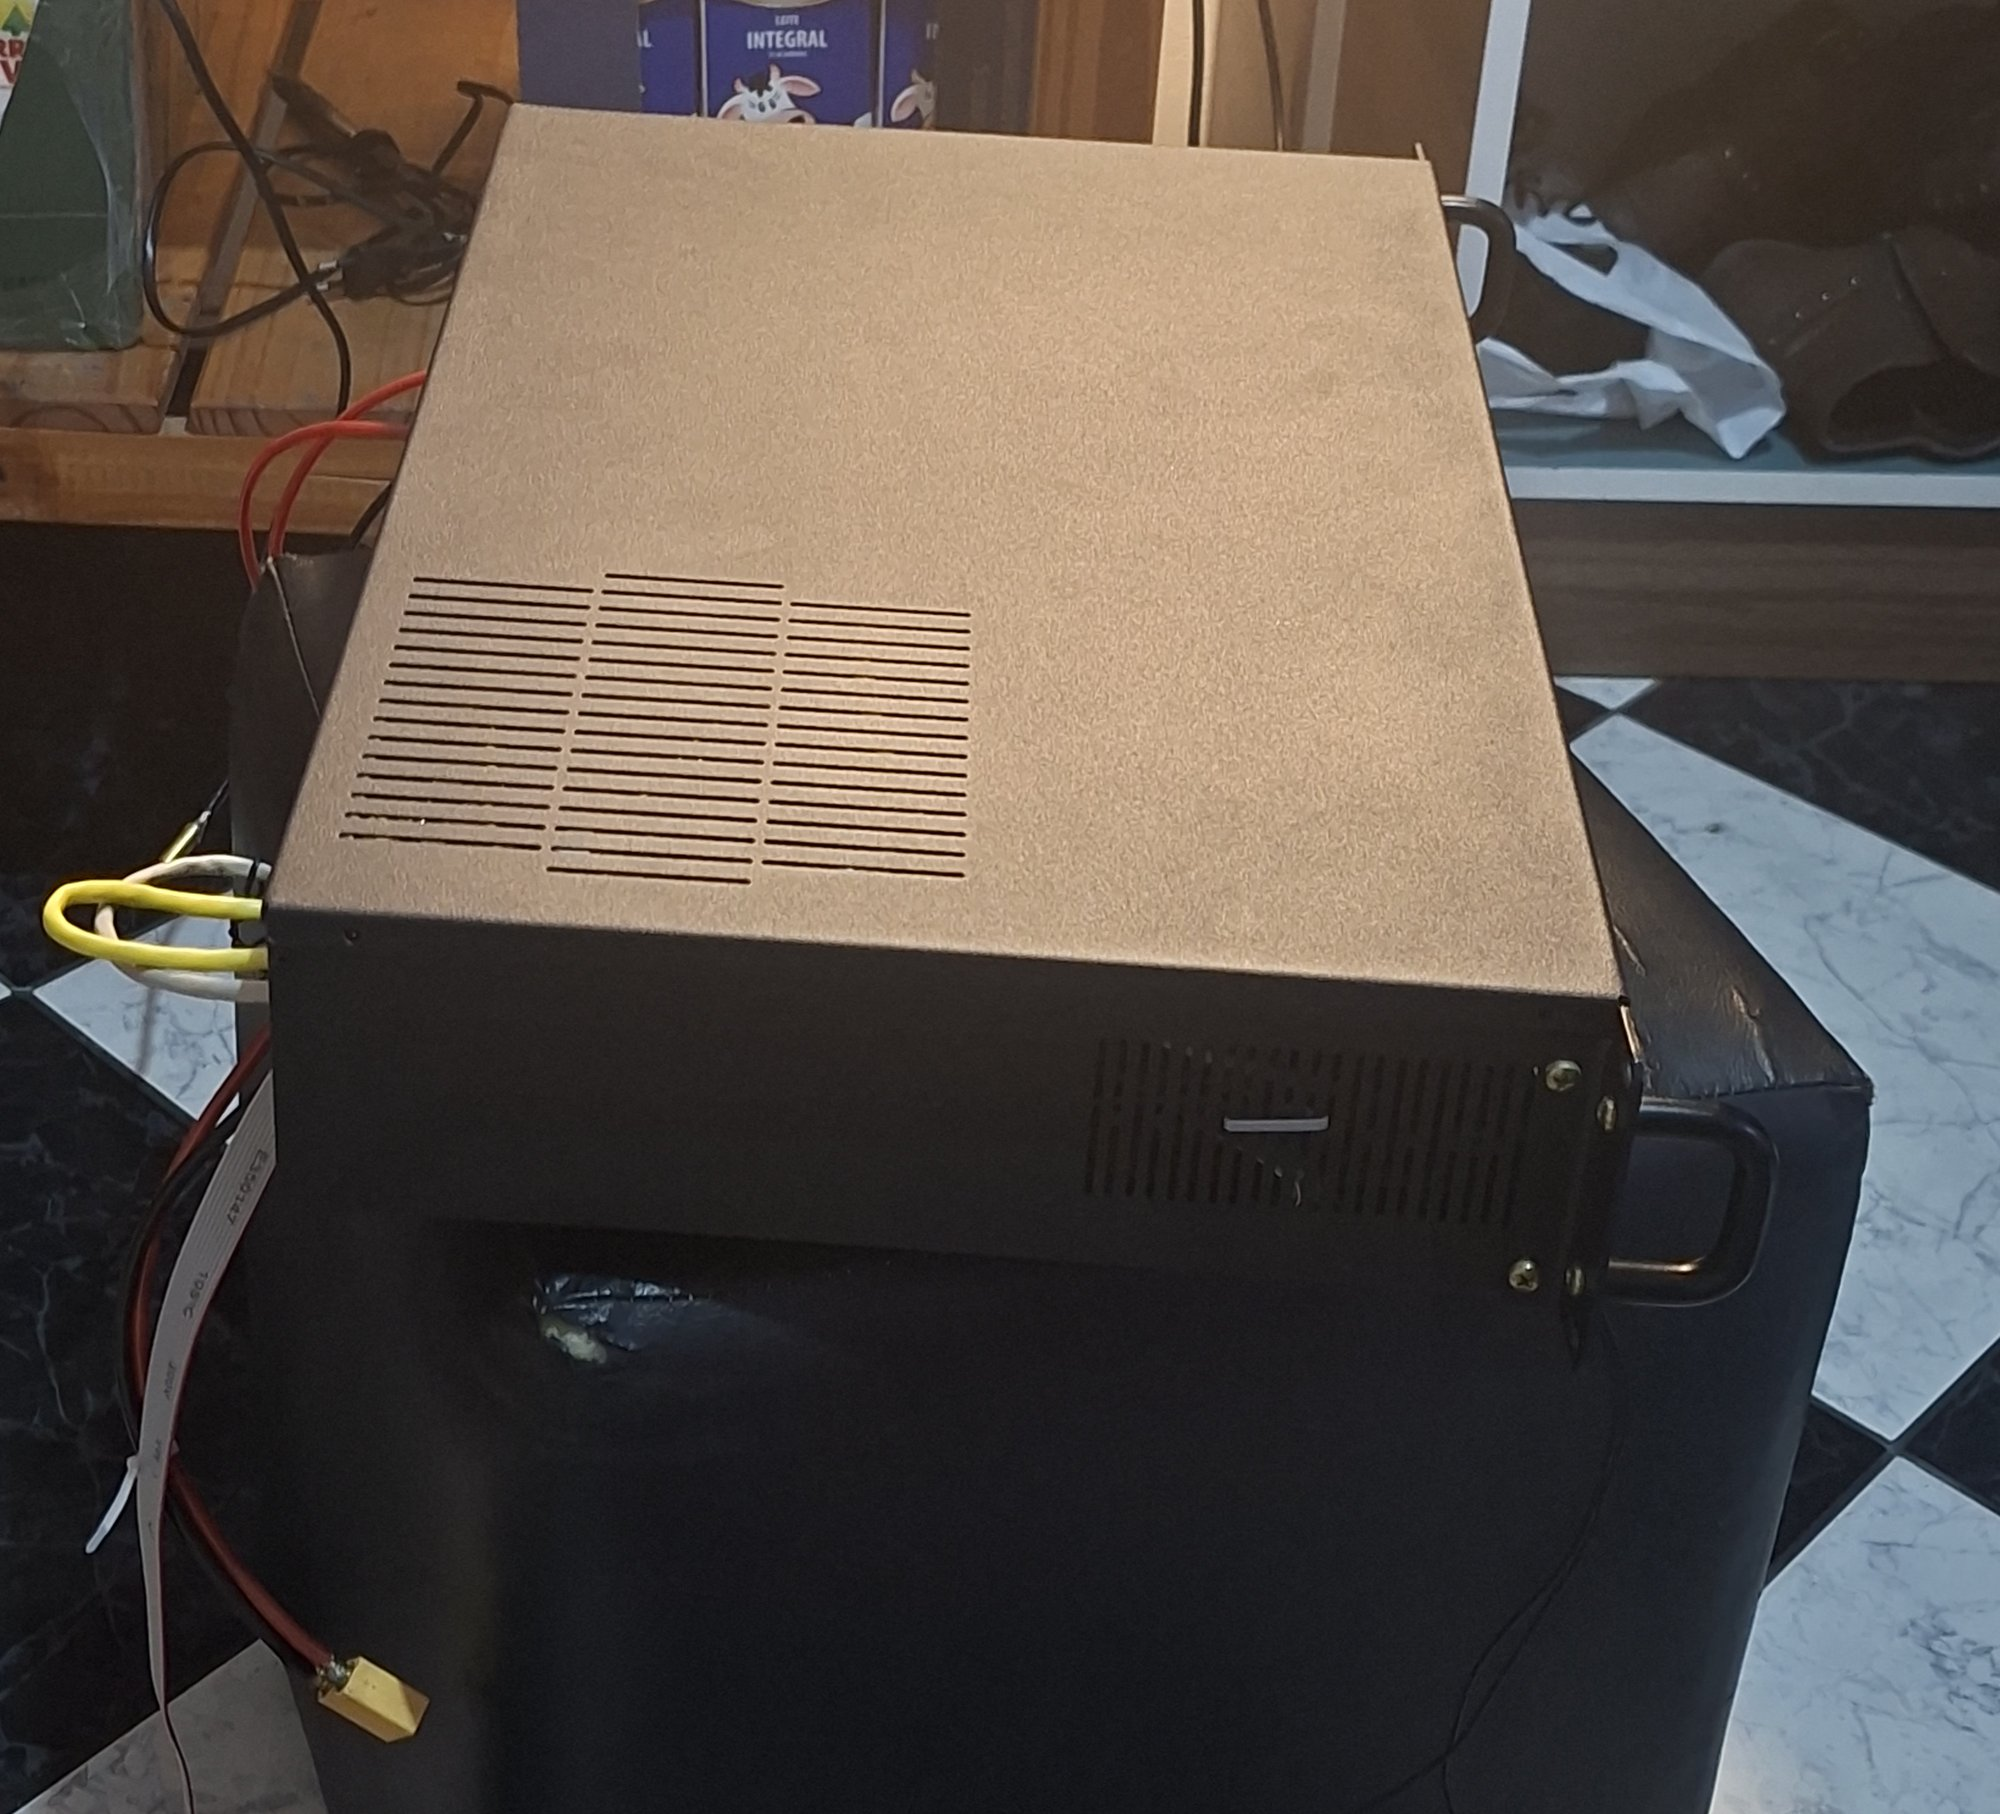
\includegraphics[height=0.5\textheight,width=0.95\linewidth,keepaspectratio]{Metodologia/gabinete.jpg}\\[0.3em]
      {\small Gabinete}
    \end{column}
  \end{columns}
  \vspace{0.6em}
  \fonte[Autor; Nanjing Qinheng Microelectronics (2026); Northrup (2018)]
\end{frame}

\begin{frame}{Firmware}
  \begin{columns}[c]
    \begin{column}{0.4\textwidth}
      \begin{itemize}
        \item Zephyr RTOS em CH32V307
        \item Fila de trabalho única
        \item Mesmo núcleo para SIBA e SAME
      \end{itemize}
    \end{column}
    \begin{column}{0.6\textwidth}
      \centering
      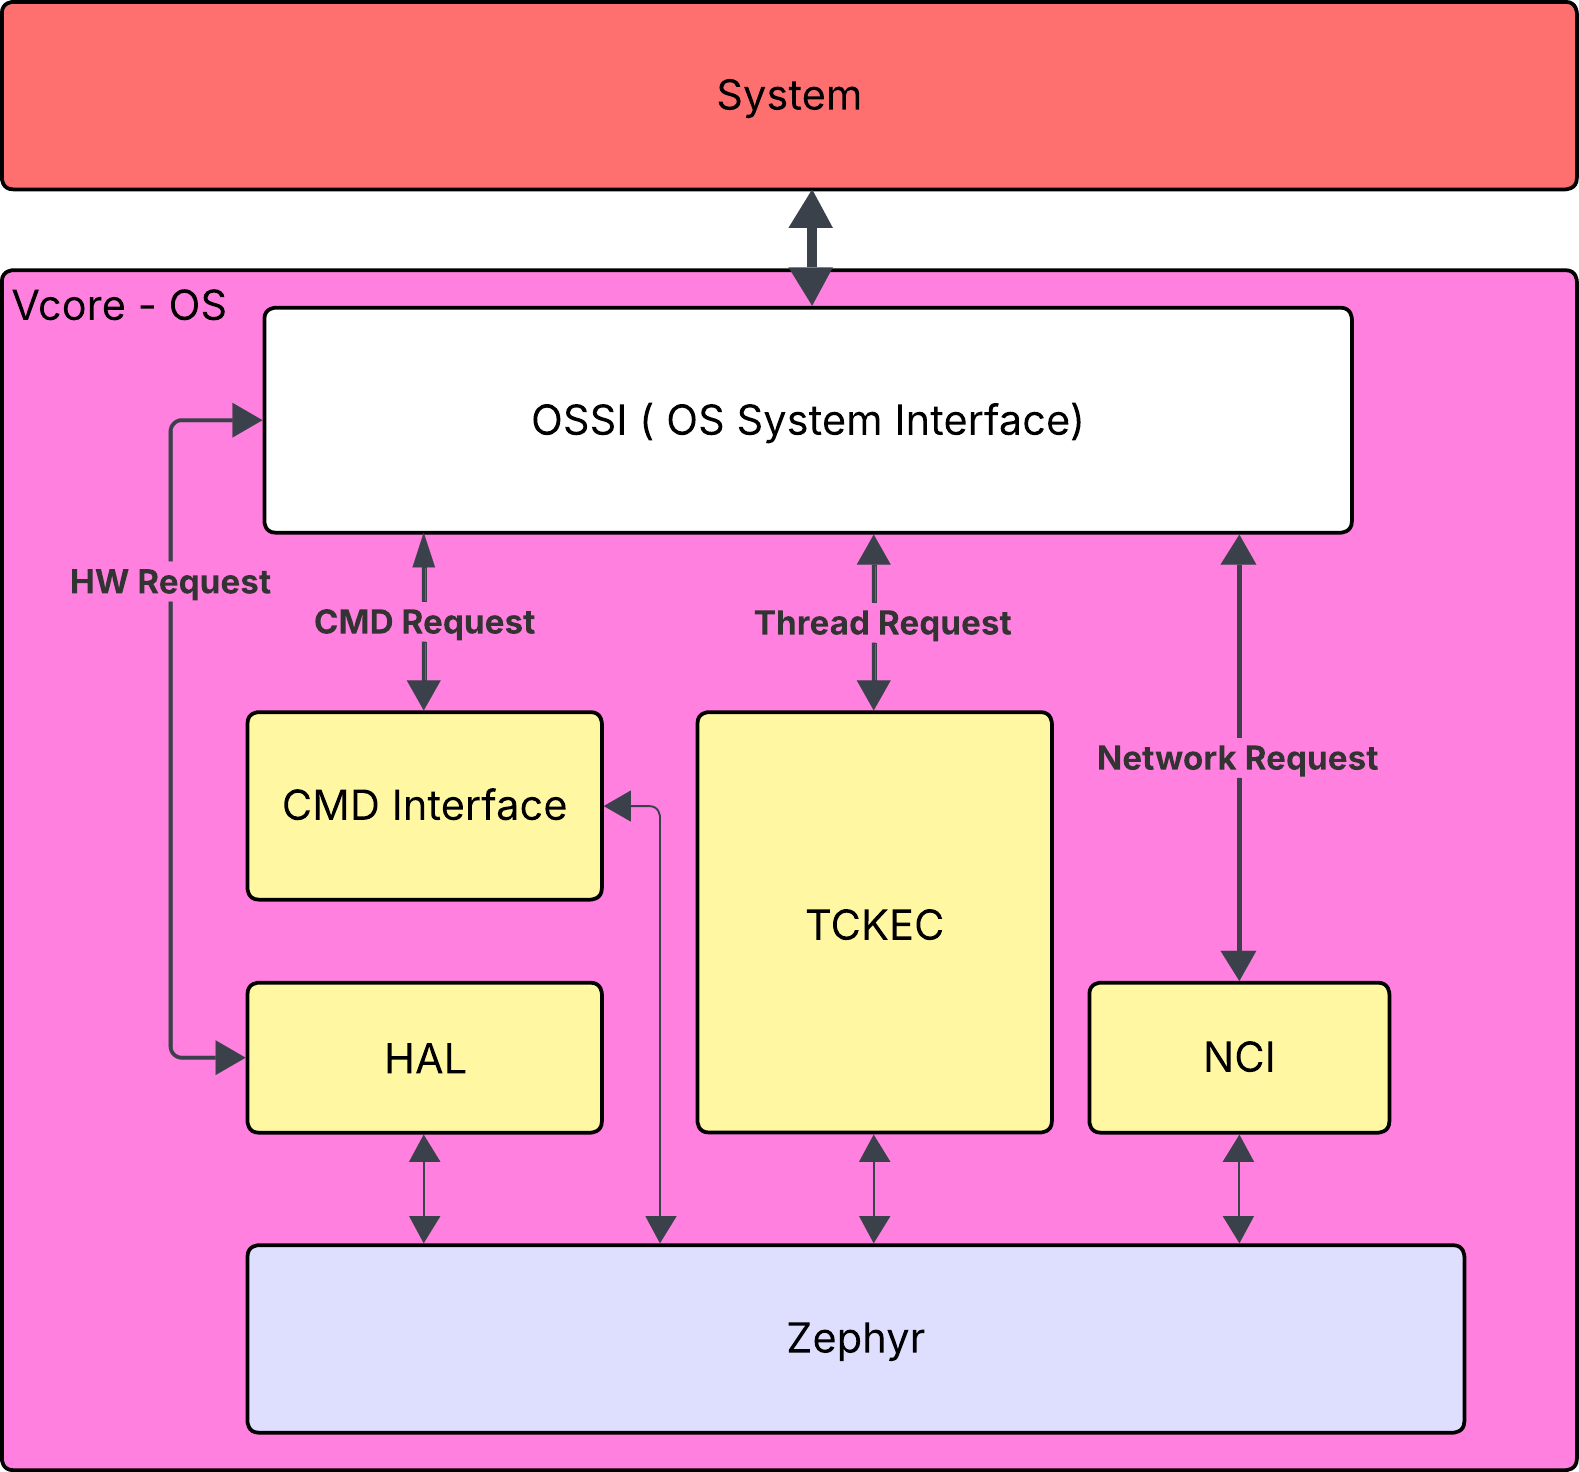
\includegraphics[height=0.72\textheight]{Metodologia/Vcore.png}
      \fonte[Adaptado de Zephyr Project (2026a; 2026b)]
    \end{column}
  \end{columns}
\end{frame}

\begin{frame}{Supervisório}
  \begin{columns}[c]
    \begin{column}{0.62\textwidth}
      \centering
      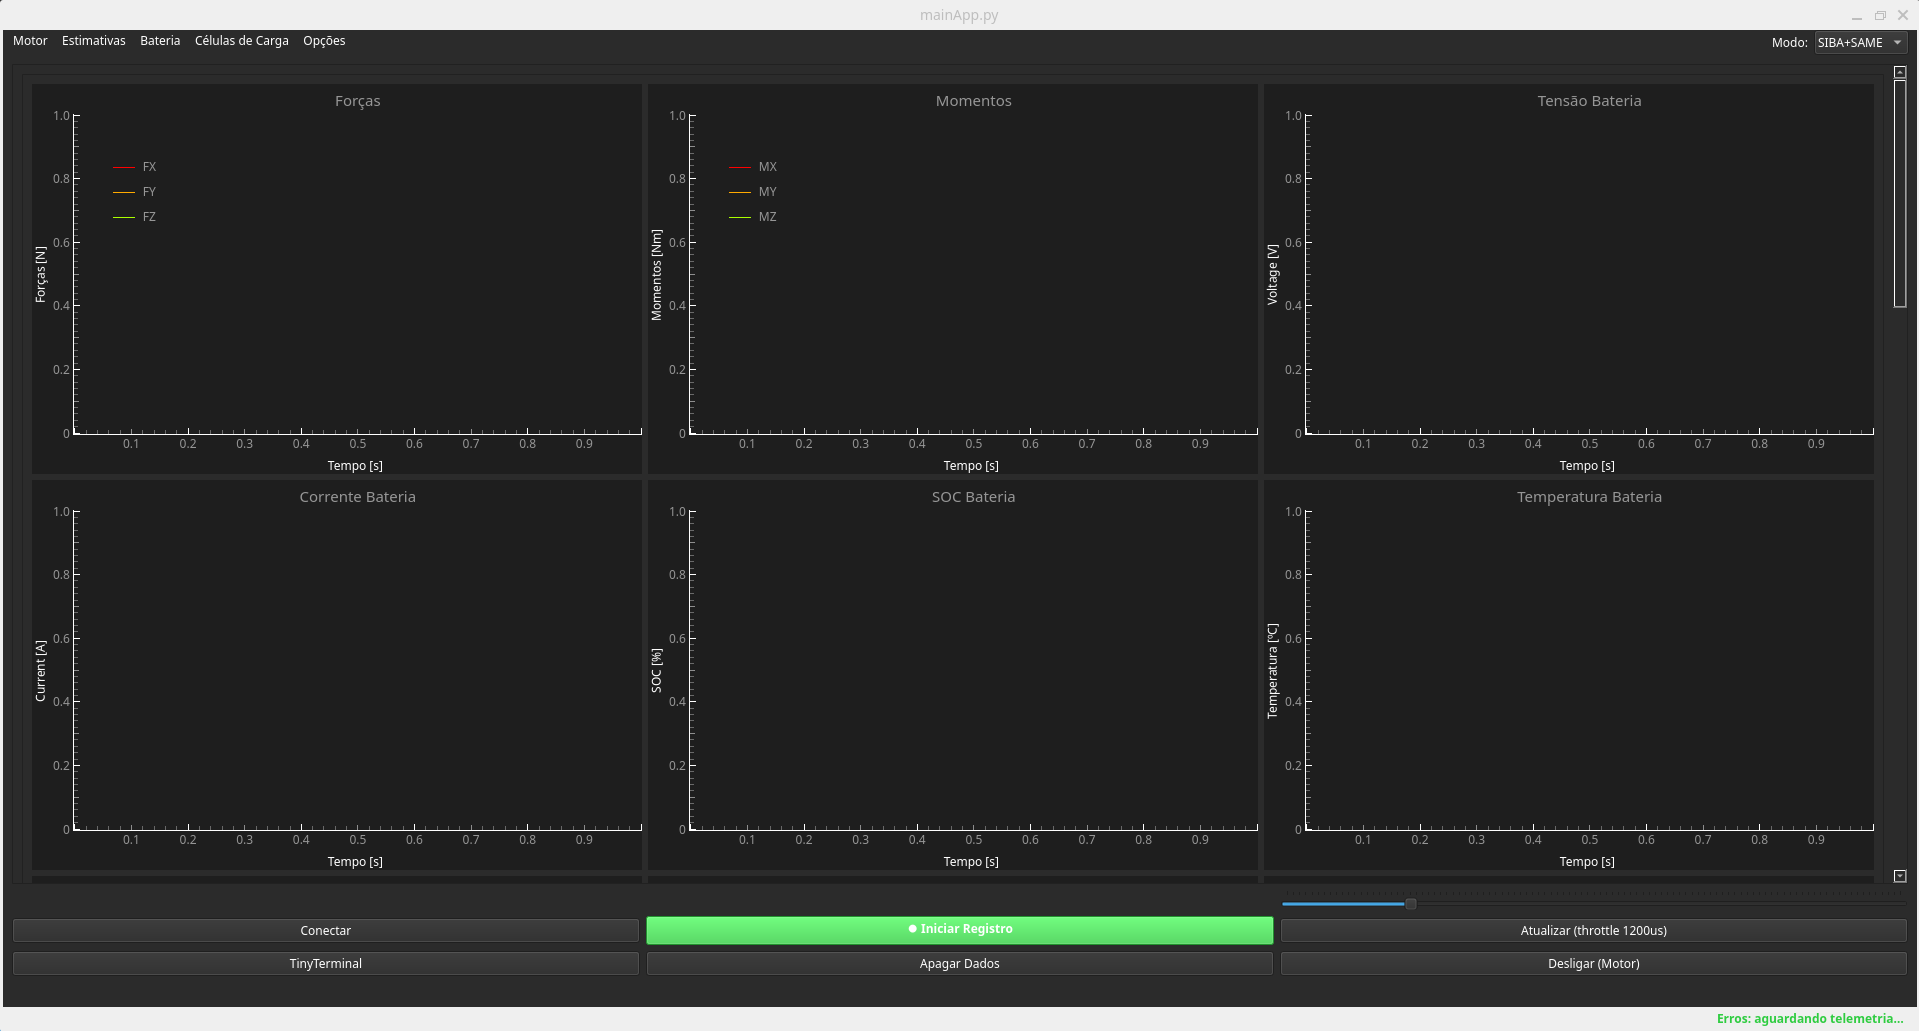
\includegraphics[width=\linewidth]{Metodologia/gui tela principal.png}
      \fonte
    \end{column}
    \begin{column}{0.38\textwidth}
      \centering
      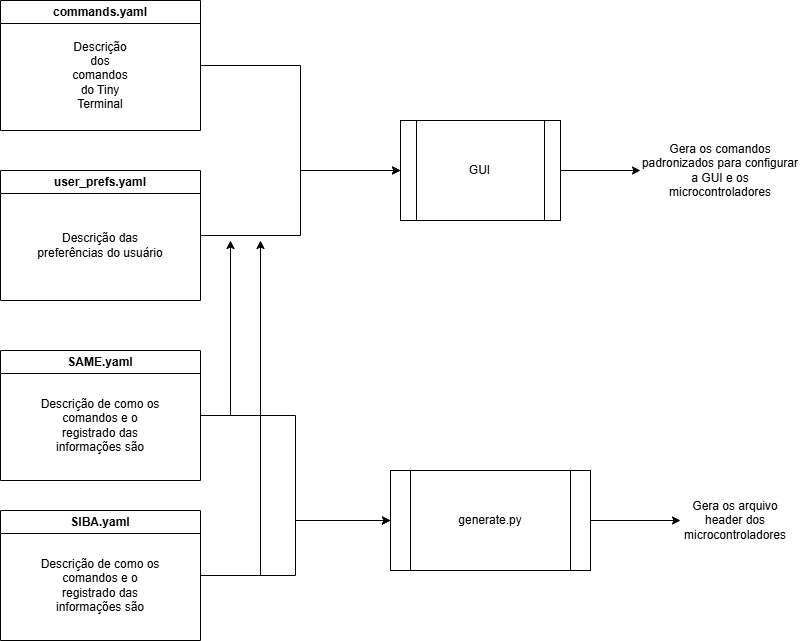
\includegraphics[width=0.85\linewidth]{Metodologia/YAML_uso.drawio.png}\\[0.3em]
      {\small YAML como fonte única para GUI e firmware}
    \end{column}
  \end{columns}
\end{frame}

%%=====================================================================
%% RESULTADOS
%% Slides com \ilustrativo trazem dados provisórios: substituir.
%%=====================================================================
\secaoudesc{Resultados}

\begin{frame}{Parâmetros elétricos}
  \begin{columns}[c]
    \begin{column}{0.5\textwidth}
      \begin{itemize}
        \item Resistência por quatro fios (Kelvin)
        \item Indutância por ressonância LC
        \item Ensaios independentes convergentes
      \end{itemize}
    \end{column}
    \begin{column}{0.5\textwidth}
      \centering
      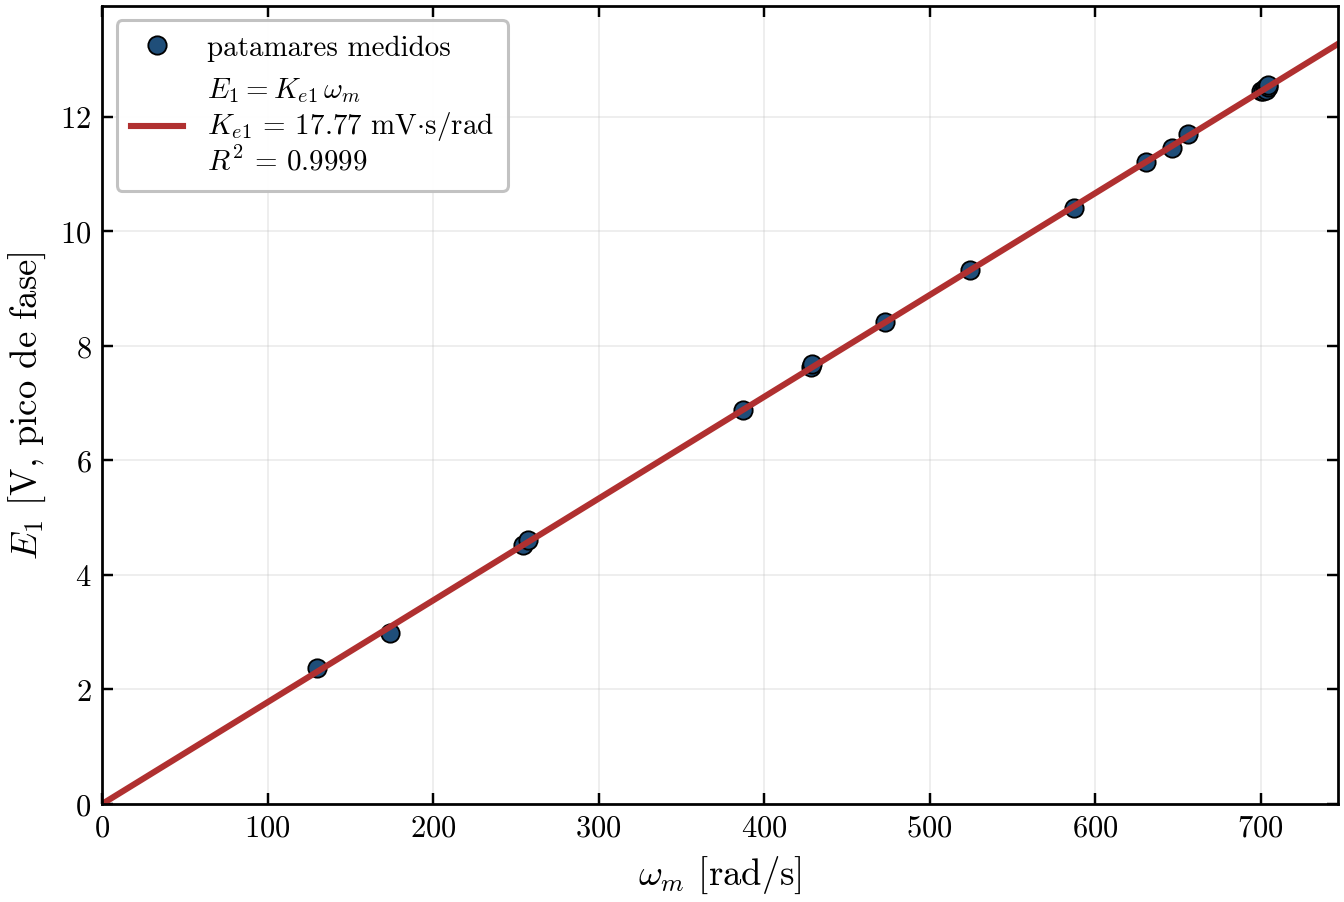
\includegraphics[width=\linewidth]{Resultados/bancada_ke.png}
      \fonte[Autor; Fitzgerald, Kingsley e Umans (2014)]
    \end{column}
  \end{columns}
\end{frame}

\begin{frame}{Perdas mecânicas}
  \begin{columns}[c]
    \begin{column}{0.36\textwidth}
      \begin{itemize}
        \item Ensaio em vazio
        \item Balanço de potência por fase
        \item Atrito viscoso e seco
      \end{itemize}
    \end{column}
    \begin{column}{0.64\textwidth}
      \centering
      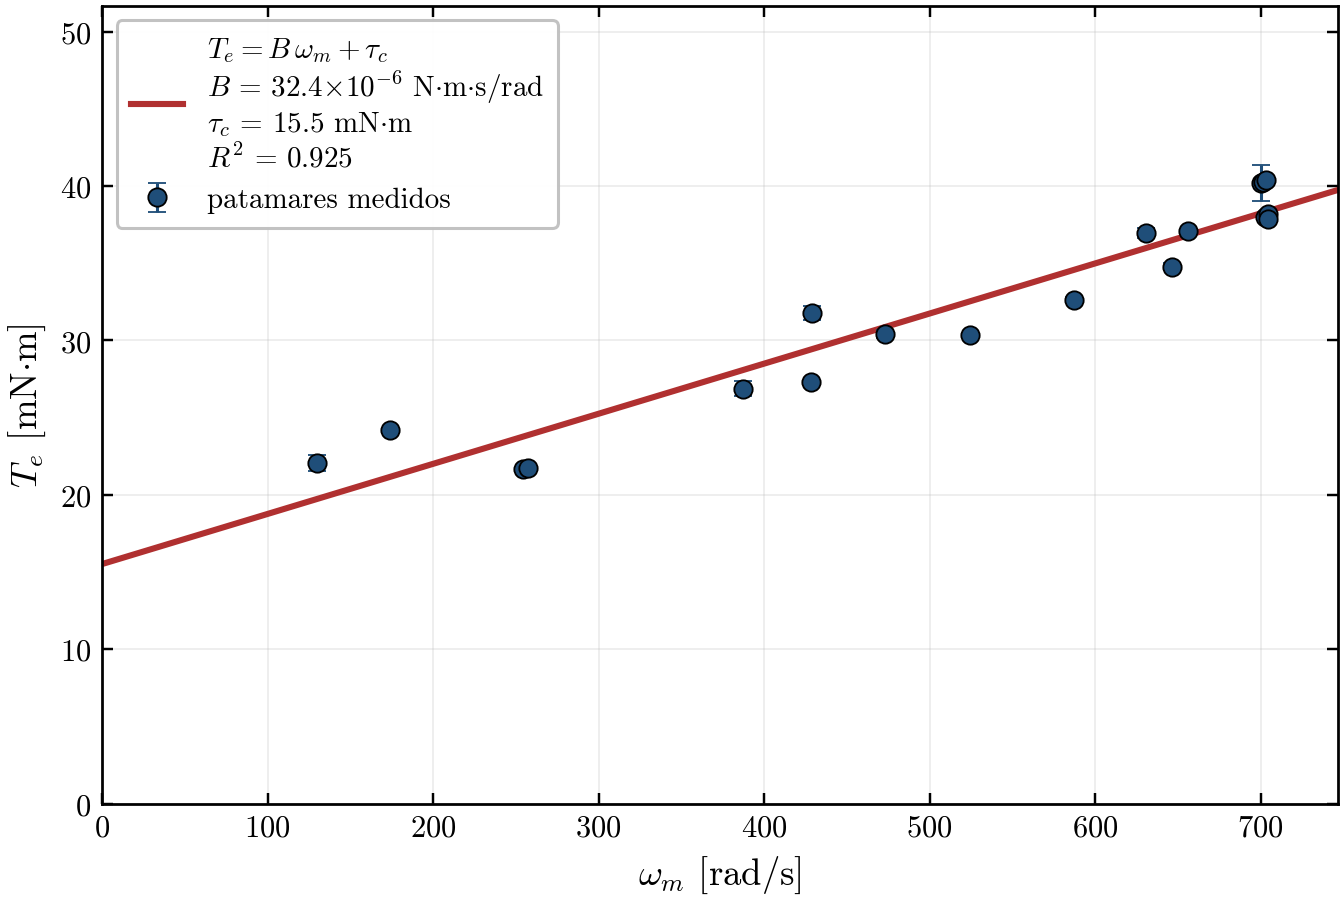
\includegraphics[width=\linewidth]{Resultados/bancada_te_omega.png}
      \fonte[Autor; Krishnan (2017)]
    \end{column}
  \end{columns}
\end{frame}

\begin{frame}{Observador em bancada}
  \begin{columns}[c]
    \begin{column}{0.36\textwidth}
      \begin{itemize}
        \item Rotação acompanha o tacômetro
        \item Ângulo coerente com os pulsos
        \item Limite em baixa rotação
      \end{itemize}
    \end{column}
    \begin{column}{0.64\textwidth}
      \centering
      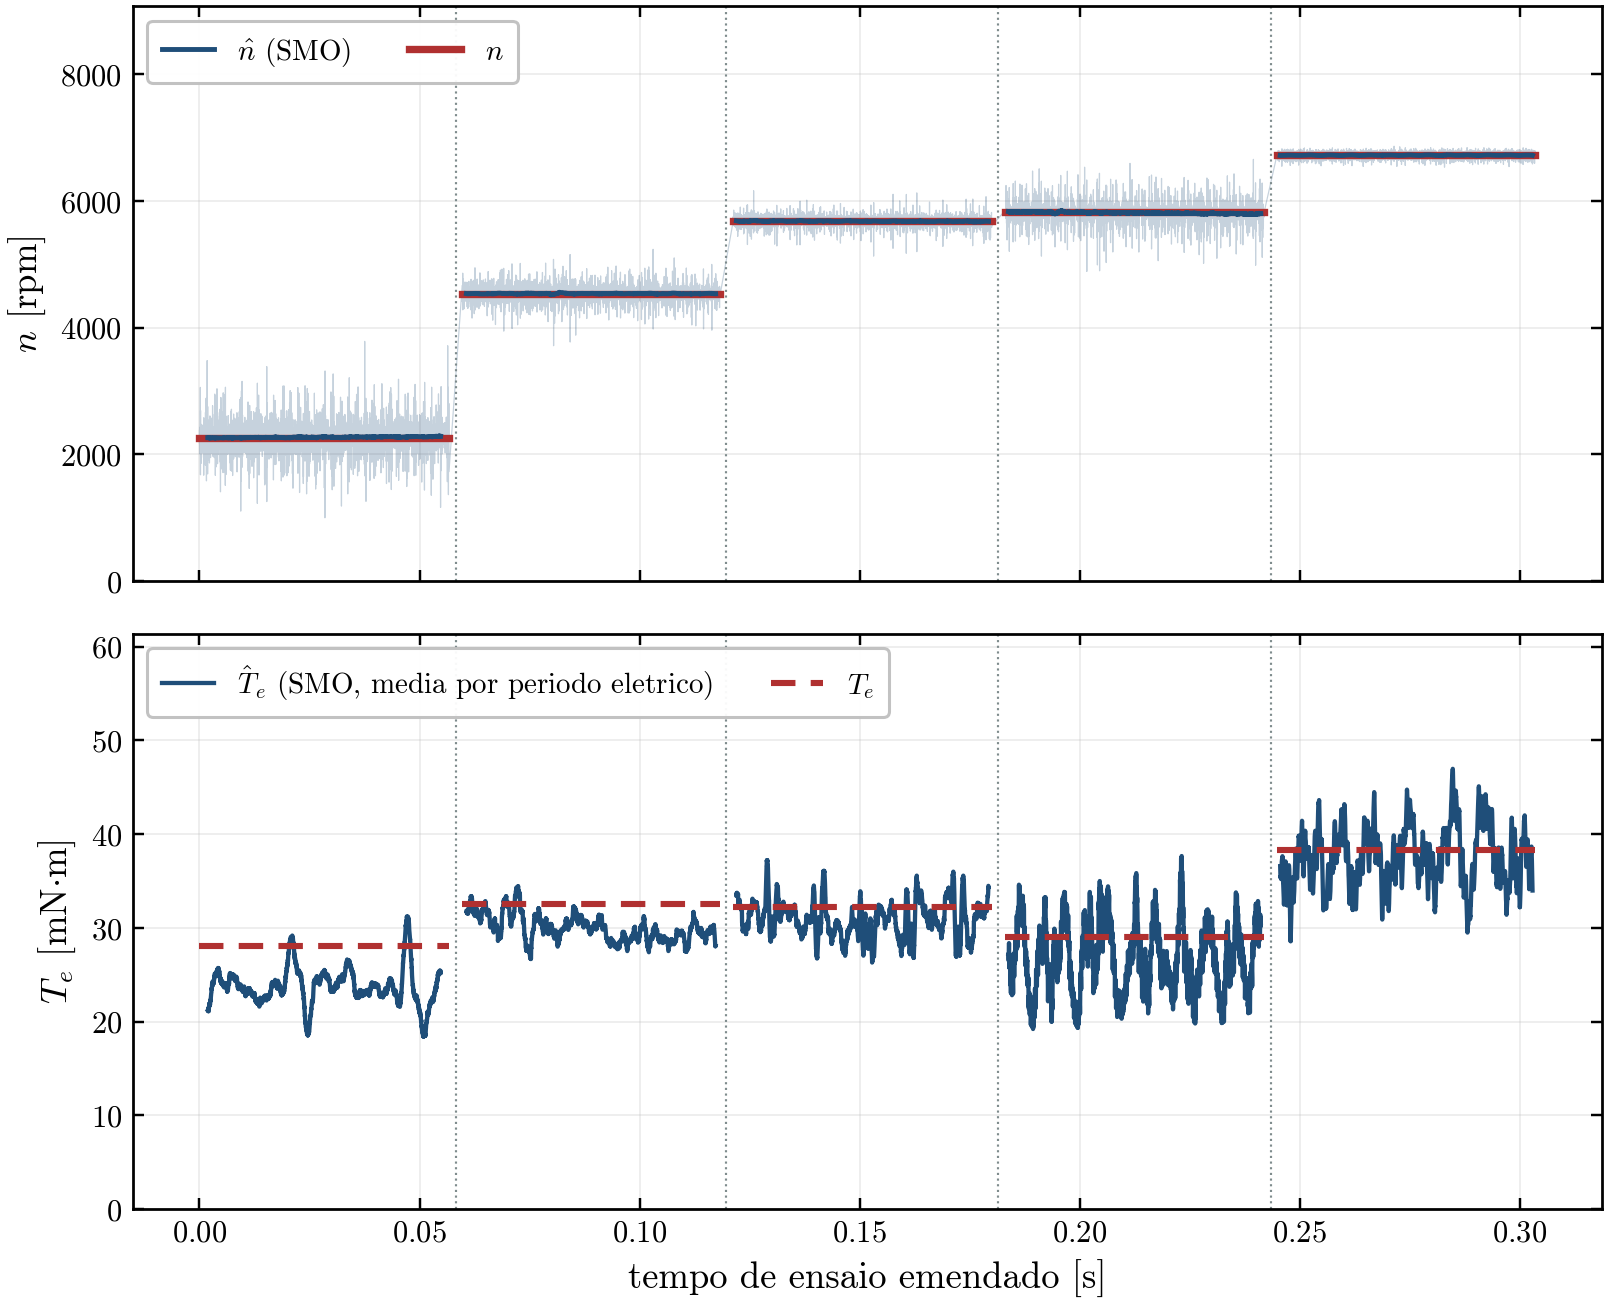
\includegraphics[height=0.72\textheight]{Resultados/bancada_smo_rpm_torque.png}
      \fonte[Autor; Nidec (2026)]
    \end{column}
  \end{columns}
\end{frame}

\begin{frame}{Torque da hélice}
  \begin{columns}[c]
    \begin{column}{0.36\textwidth}
      \begin{itemize}
        \item Duas hélices APC
        \item $C_Q$ estimado só com grandezas elétricas
        \item Comparado ao fabricante
      \end{itemize}
    \end{column}
    \begin{column}{0.64\textwidth}
      \centering
      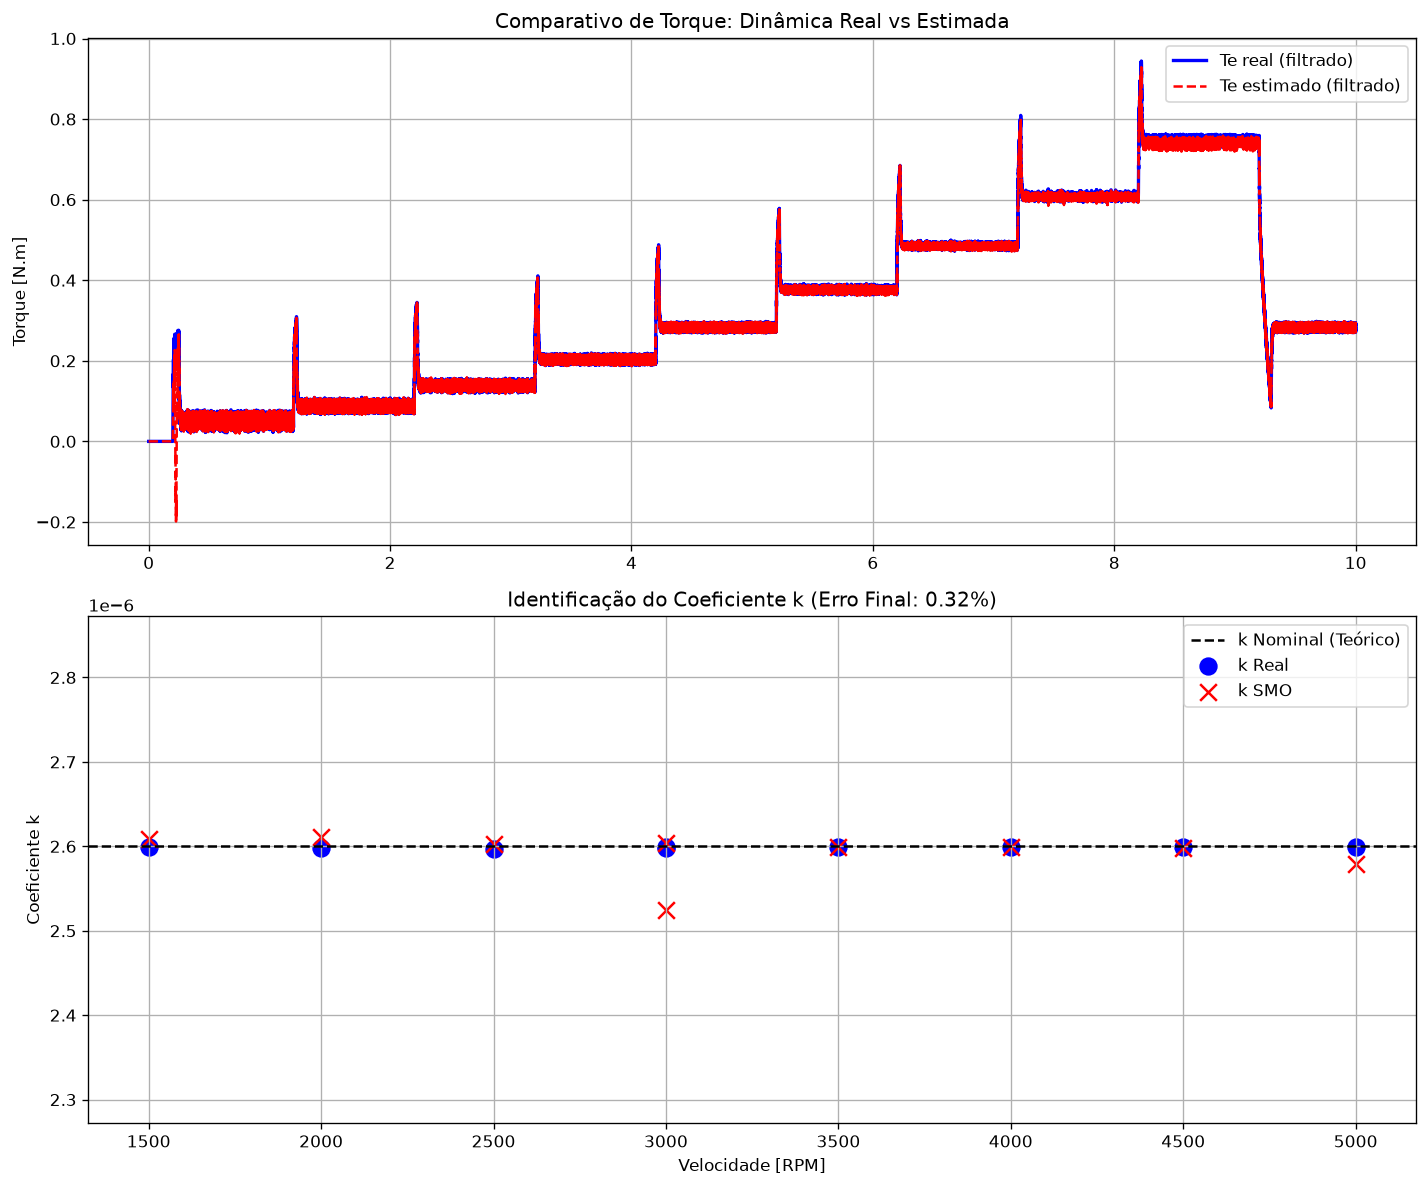
\includegraphics[height=0.72\textheight]{Desenvolvimento/Algortimo_Coeficiente_helice_17x10E.png}
      \fonte[Autor; APC Propellers (2026); Selig (2026); McCormick (1995)]
    \end{column}
  \end{columns}
\end{frame}

%% ----- a partir daqui: RESULTADOS ILUSTRATIVOS (substituir) -----

\begin{frame}{Validação da SIBA}
  \ilustrativo
  \centering
  \begin{tabular}{lc}
    \toprule
    \textbf{Sensor} & \textbf{Erro vs. referência} \\
    \midrule
    Tensão da bateria   & Dentro da tolerância \\
    Corrente da bateria & Dentro da tolerância \\
    Células de carga    & Dentro da tolerância \\
    Tubo de Pitot       & Dentro da tolerância \\
    \bottomrule
  \end{tabular}
  \fonte[Autor; Northrup (2018); Brandt et al.\ (2015)]

  \destaque{Cadeia aerodinâmica dentro da faixa exigida pela equipe.}
\end{frame}

\begin{frame}{Ensaio integrado}
  \ilustrativo
  \begin{columns}[c]
    \begin{column}{0.36\textwidth}
      \begin{itemize}
        \item SIBA e SAME sincronizadas
        \item Tração, torque e rotação no mesmo registro
        \item Exportação em CSV
      \end{itemize}
    \end{column}
    \begin{column}{0.64\textwidth}
      \centering
      \placeholder{8.5cm}{5.2cm}{Tração e torque estimado\\em função da rotação\\(ensaio integrado)}
      \fonte
    \end{column}
  \end{columns}
\end{frame}

%%=====================================================================
%% CONCLUSÃO
%% Redigida assumindo a validação integrada concluída com sucesso;
%% revisar quando os resultados ilustrativos forem substituídos.
%%=====================================================================
\secaoudesc{Conclusão}

\begin{frame}{Conclusão}
  \begin{itemize}
    \item Bancada integrada e operacional
    \item Torque e rotação sem sensor mecânico
    \item Grandezas elétricas e aerodinâmicas no mesmo registro
    \item Procedimento repetível para novos conjuntos
  \end{itemize}

  \destaque{Escolha de motor e hélice apoiada em ensaio próprio.}
\end{frame}

\begin{frame}{Trabalhos futuros}
  \begin{itemize}
    \item Dinamômetro para torque de referência
    \item Curva SOC $\times$ OCV da bateria
    \item Efeito da temperatura da bateria na tração
    \item Observador em enfraquecimento de campo
    \item Bancada com 6 graus de liberdade
  \end{itemize}
\end{frame}

%%=====================================================================
%% REFERÊNCIAS (ABNT, extraídas de ../Textual/abntex2-ref_UDESC_2020.bib)
%%=====================================================================
\begin{frame}{Referências}
  \tiny
  \setlength{\parskip}{0.35em}

  ABO KAF, A. \textit{et al.} Sensorless direct torque control in brushless
  DC motor using sliding mode observer. In: INTERNATIONAL CONFERENCE ON
  EMERGING SMART TECHNOLOGIES AND APPLICATIONS (eSmarTA), 4., 2024.
  \textbf{Anais} [...]. IEEE, 2024.

  APC PROPELLERS. \textbf{Performance data}. 2026. Disponível em:
  https://www.apcprop.com/technical-information/performance-data/.

  BRANDT, S. A. \textit{et al.} \textbf{Introduction to aeronautics}: a
  design perspective. 3. ed. AIAA Education Series, 2015.

  FITZGERALD, A. E.; KINGSLEY, C.; UMANS, S. D. \textbf{Máquinas
  elétricas}. 7. ed. Porto Alegre: Bookman, 2014.

  KRISHNAN, R. \textbf{Permanent magnet synchronous and brushless DC motor
  drives}. Boca Raton: CRC Press, 2017.

  McCORMICK, B. W. \textbf{Aerodynamics, aeronautics, and flight
  mechanics}. 2. ed. New York: John Wiley \& Sons, 1995.

  SAE BRASIL. \textbf{Regulamento SAE Brasil Aerodesign 2024}. São Paulo,
  2024.

  SELIG, M. S. \textbf{UIUC propeller database}. 2026. Disponível em:
  https://m-selig.ae.illinois.edu/props/propDB.html.

  SOUZA, L. C.; VEBER, W. C. P. \textbf{Desempenho -- Nº 012}: Albatroz
  Aerodesign. Joinville: UDESC, 2023. Relatório técnico.

  UTKIN, V. I. \textbf{Sliding modes in control and optimization}. Berlin:
  Springer-Verlag, 1992.

  ZEPHYR PROJECT. \textbf{Zephyr Project documentation}: scheduling,
  interrupts, and synchronization. 2026. Disponível em:
  https://docs.zephyrproject.org.
\end{frame}


\fechamentoudesc

\end{document}
